\documentclass[conference]{IEEEtran}
\IEEEoverridecommandlockouts

% Core packages
\usepackage{cite}
\usepackage{amsmath,amssymb,amsfonts}
\usepackage{algorithmic}
\usepackage{graphicx}
\usepackage{textcomp}
\usepackage{xcolor}
\usepackage{float}

% Additional packages
\usepackage{booktabs}
\usepackage{hyperref}
\usepackage{enumitem}
\usepackage{tabularx}
\usepackage{multirow}

\usepackage{listings}
\usepackage[htt]{hyphenat}

\lstset{
  basicstyle=\ttfamily\small,
  breaklines=true,
  breakatwhitespace=true,
  postbreak=\mbox{\textcolor{gray}{$\hookrightarrow$}\space},
  numbers=none,
  frame=single,
  captionpos=b,
  tabsize=2,
  showstringspaces=false
}

\begin{document}

\title{Community Detection and Recommendation Systems in Product Co-Purchasing Networks}

\author{
\IEEEauthorblockN{Muhammad Fauzan Jaisyurrahman - 2206814040 \\ 
Muhammad Nabiel Subhan - 2206081553 \\ 
Hanan Adipratama - 2206081824 \\ 
Kevin Ignatius Wijaya - 2206083470 \\ 
Iqza Ardiansyah - 2206810042}
\IEEEauthorblockA{\textit{Fakultas Ilmu Komputer} \\
\textit{Universitas Indonesia}\\
Depok, Indonesia}
}

\maketitle

\begin{abstract}
E-commerce platforms leverage complex networks of product relationships formed through co-purchasing behaviors. This paper applies network science methodologies to analyze product co-purchasing patterns using the CRISP-DM framework. We constructed a graph representation with 259,102 products (nodes) and 879,700 co-purchasing relationships (edges), then applied the Louvain community detection algorithm to identify meaningful product communities. Our analysis revealed a structured network with 190 distinct communities representing coherent product categories. We developed and evaluated three recommendation approaches: basic neighbor-based, community-aware, and an advanced model incorporating popularity metrics. Both basic and community-aware approaches achieved identical high precision (0.9960), while the advanced model showed slightly lower precision (0.8920) but potentially greater recommendation diversity. Through empirical evaluation using a sample of influential products, we observed that recommendations within the same community exhibited stronger contextual relevance despite similar quantitative metrics. This research demonstrates how community detection can enhance product recommendation strategies, potentially increasing cross-selling opportunities and customer satisfaction in e-commerce platforms.
\end{abstract}

\section{Introduction}
In the evolving landscape of e-commerce, understanding product relationships and customer purchasing patterns has become increasingly important for businesses seeking to maximize sales and enhance customer experiences. When customers browse online stores, they often purchase multiple items together, creating implicit relationships between products. These relationships form a complex network structure that can be analyzed using graph theory and network science principles \cite{linden2003amazon}.

This research leverages the Cross-Industry Standard Process for Data Mining (CRISP-DM) methodology to analyze a product co-purchasing network. The CRISP-DM framework provides a structured approach to data mining projects, breaking them down into six phases: business understanding, data understanding, data preparation, modeling, evaluation, and deployment \cite{shearer2000crisp}. This methodology is particularly suitable for our problem as it emphasizes the importance of understanding the business context before diving into the technical implementation.

\subsection{Research Motivation and Objectives}
The motivation for this research stems from the need for improved recommendation systems in e-commerce platforms. Traditional recommendation approaches often focus solely on individual product characteristics or user-product interactions, potentially missing the valuable information embedded in product co-purchasing networks \cite{sarwar2001item}.

Our primary objectives are:
\begin{itemize}
    \item To construct and analyze a product co-purchasing network to understand its structural properties
    \item To identify natural communities of products that are frequently purchased together
    \item To develop and evaluate recommendation strategies that leverage community structure
    \item To assess how community-aware recommendations compare to traditional approaches
\end{itemize}

By achieving these objectives, we aim to provide insights that can lead to more contextually relevant product recommendations, potentially increasing cross-selling opportunities and improving customer satisfaction.

\subsection{Related Work}
Research on network analysis for recommendation systems has gained significant attention in recent years. Huang et al. \cite{huang2007applying} demonstrated the value of using association rules and collaborative filtering techniques for mining co-purchase patterns in e-commerce. Their work, however, did not explicitly explore the community structure of product networks.

Community detection in complex networks has been studied extensively, with numerous algorithms proposed for identifying cohesive subgroups. The Louvain method for community detection, developed by Blondel et al. \cite{blondel2008fast}, has gained popularity due to its computational efficiency and effectiveness in identifying hierarchical community structures in large networks. This method optimizes modularity, a measure that quantifies the density of connections within communities compared to connections between communities.

Recommendation systems have evolved from simple collaborative filtering approaches to more sophisticated models incorporating various data sources and methodologies \cite{ricci2011introduction}. Hybrid recommendation systems, which combine multiple techniques, have shown promise in addressing the limitations of individual approaches \cite{burke2002hybrid}. However, the explicit incorporation of community structure in product networks remains relatively underexplored in the recommendation system literature.

More recently, Shokrzadeh et al.\ \cite{shokrzadeh2022graph} proposed a graph-based recommendation pipeline that first applies the Louvain community detection on a tag-similarity graph and then scores items by community membership; they report up to a 7\% relative gain in precision and recall on two public datasets. Their results reaffirm that explicitly integrating community structure into recommendation algorithms can meaningfully improve accuracy and diversity.

Our work builds upon these foundations by explicitly integrating community detection with product recommendation strategies. Unlike previous studies that primarily focus on either network analysis or recommendation systems in isolation, we bridge these domains to develop community-aware recommendation strategies and empirically evaluate their performance.

The implementation of data preparation, community detection, and recommendation evaluation is available at our GitHub repository: https://github.com/hanan-collab/Community-Aware-Product-Recommendation-using-Louvain-Algorithm-on-Amazon-Co-Purchasing-Network \cite{repo}.

\section{Business and Data Understanding}
\subsection{Business Context and Objectives}
The primary business objective of this research is to enhance product recommendation systems for e-commerce platforms by leveraging network structure and community detection. Effective recommendation systems can significantly impact key business metrics such as:

\begin{itemize}
    \item \textbf{Conversion rates:} By suggesting relevant products, retailers can increase the likelihood of purchases
    \item \textbf{Average order value:} Appropriate product recommendations can encourage customers to add more items to their carts
    \item \textbf{Customer satisfaction:} Contextually relevant recommendations enhance the shopping experience
    \item \textbf{Customer retention:} Personalized shopping experiences can increase customer loyalty
\end{itemize}

Key stakeholders for this research include e-commerce platform managers, marketing teams, and data scientists responsible for designing and implementing recommendation systems. The expected benefits include improved recommendation quality, increased cross-selling opportunities, and enhanced customer experience, while potential risks involve recommendations that might be perceived as irrelevant or intrusive.

\subsection{Dataset Description}
This study utilizes the Amazon Product Co-Purchasing Network dataset, which was collected from Amazon.com. The dataset is publicly available and has been widely used in research involving product recommendation, graph-based analysis, and consumer behavior modeling. It contains two main components:

\begin{enumerate}
    \item \textbf{Products data:} Contains information about 259,167 unique products, including attributes such as product ID, title, category (group), sales rank, review count, number of downloads, rating, and network connectivity metrics.
    
    \item \textbf{Co-purchase data:} Contains 1,207,337 directed edges representing co-purchasing relationships between products. Each edge indicates that when a customer purchased the "source" product, they also purchased the "target" product.
\end{enumerate}

Table \ref{tab:data-summary} provides an overview of the dataset dimensions.

\begin{table}[ht]
\centering
\caption{Dataset Summary}
\label{tab:data-summary}
\begin{tabular}{lc}
\toprule
\textbf{Attribute} & \textbf{Value} \\
\midrule
Number of products (nodes) & 259,167 \\
Number of co-purchases (edges) & 1,207,337 \\
Features available & id, title, group, salesrank, \\
 & review\_cnt, downloads, rating, \\
 & outgoing\_count, incoming\_count, \\
 & total\_connections \\
\bottomrule
\end{tabular}
\end{table}

This dataset allows us to model the co-purchasing behavior as a directed graph where nodes represent products and edges represent co-purchasing relationships. By analyzing this graph, we can uncover patterns in customer purchasing behavior and identify communities of products that are frequently purchased together.

\subsection{Preliminary Data Analysis}
Initial analysis of the graph structure revealed several interesting properties:

\begin{itemize}
    \item \textbf{Network density:} The graph is sparse, with a density significantly lower than 1, indicating that most products are co-purchased with only a small subset of other products.
    
    \item \textbf{Clustering coefficient:} The average clustering coefficient suggests the presence of local clusters in the network, indicating that products tend to form small, densely connected groups.
    
    \item \textbf{Degree distribution:} The network exhibits a heavy-tailed degree distribution, with a small number of products having very high connectivity (hub products) while most products have relatively few connections.
\end{itemize}

These properties suggest that the product co-purchasing network has a complex structure with natural communities, making it suitable for community detection and network-based recommendation approaches.

\section{Data Preparation}
Data preparation is a crucial step in the CRISP-DM methodology, ensuring that the data is in a suitable form for analysis. In this section, we describe the steps taken to prepare the co-purchasing data for network analysis and community detection.

\subsection{Data Cleaning and Preprocessing}
The data preparation process involved several steps to ensure the quality and integrity of the dataset:

\begin{enumerate}
    \item \textbf{Handling missing values:} We identified and removed rows with missing values in the Source or Target columns of the co-purchase dataset, as these are essential for constructing the network. For the products dataset, we filled missing numerical values with appropriate measures of central tendency and replaced missing categorical values with placeholders.
    
    \item \textbf{Removing duplicates:} Duplicate co-purchasing relationships were eliminated to prevent overrepresentation of certain product pairs.
    
    \item \textbf{Data type consistency:} We ensured that product IDs were consistently represented as strings across both datasets to facilitate proper joining of information.
    
    \item \textbf{Validation:} We verified that all products referenced in the co-purchase data existed in the products dataset, removing any references to non-existent products.
    
    \item \textbf{Handling self-loops:} Co-purchasing relationships where a product referenced itself were removed as they do not represent meaningful relationships for our analysis.
\end{enumerate}

The resulting cleaned dataset contained no missing values and maintained referential integrity between the co-purchase and product information.

\subsection{Feature Engineering}
To enhance our understanding of product relationships in the network, we created additional features:

\begin{itemize}
    \item \textbf{Outgoing count:} The number of products that are co-purchased with each product when the product is the source
    \item \textbf{Incoming count:} The number of products that lead to the purchase of each product when the product is the target
    \item \textbf{Total connections:} The sum of incoming and outgoing connections, representing the overall connectivity of a product in the network
\end{itemize}

These features provided valuable insights into each product's position and importance in the co-purchasing network, facilitating the identification of influential products for recommendation.

\subsection{Sampling Strategy for Analysis}
\label{sec:sampling}
Given the large size of the network (259,102 nodes and 879,700 edges), certain analytical operations required careful sampling to maintain computational feasibility. To ensure reproducibility, we set fixed random seeds (42) for all stochastic operations. Our sampling strategy employed several approaches depending on the specific analytical task:

\begin{enumerate}
    \item \textbf{Clustering coefficient calculation:} For networks with more than 10,000 nodes, we randomly sampled 1,000 nodes to estimate the average clustering coefficient. This approach provides a statistically reasonable approximation while significantly reducing computation time. The sampling is implemented in the \texttt{analyze\_graph} function of our code:
    
    \begin{lstlisting}
if node_count > 10000:
    sample_size = min(1000, node_count)
    nodes_list = list(G.nodes())
    sampled_nodes = random.sample(
        nodes_list, 
        sample_size)
    results['avg_clustering'] = nx.average_clustering(
        G, 
        nodes=sampled_nodes)
    \end{lstlisting}
    
    \item \textbf{Centrality measures:} For large networks, we used degree centrality as a proxy for more computationally expensive centrality measures, focusing on the most connected nodes when identifying influential products.
    
    \item \textbf{Visualization sampling:} When visualizing the network, we limited the graph to the top 100 nodes by degree centrality rather than selecting random nodes. This approach ensures that the visualization captures the most influential parts of the network:
    
    \begin{lstlisting}
if G.number_of_nodes() > max_nodes:
    degrees = dict(G.degree())
    sorted_nodes = sorted(
        degrees.items(), 
        key=lambda x: x[1], 
        reverse=True)
    sampled_nodes = [
        node 
        for node, _ in sorted_nodes[:max_nodes]
    ]
    G_sample = G.subgraph(sampled_nodes)
    \end{lstlisting}
    
    \item \textbf{Recommendation evaluation:} When evaluating the recommendation system, we randomly selected 50 products (or fewer if the network contained fewer nodes) to serve as test cases. To ensure reproducibility, we maintained the same seed across all evaluations:
    
    \begin{lstlisting}
# Set seed for all random operations
random.seed(42)
np.random.seed(42)

# Later in the code
sample_size = min(50, len(G.nodes()))
nodes_list = list(G.nodes())
test_products = random.sample(
    nodes_list, 
    sample_size)
    \end{lstlisting}
\end{enumerate}

This strategic sampling approach with fixed random seeds allowed us to balance computational efficiency with analytical rigor, ensuring that our insights remained representative of the overall network while making the analysis computationally tractable and reproducible.

\subsection{Graph Construction}
Using the cleaned data, we constructed a directed graph where:

\begin{itemize}
    \item Nodes represent individual products
    \item Edges represent co-purchasing relationships
    \item Edge weights (where applicable) represent the strength or frequency of the co-purchasing relationship
\end{itemize}

The graph construction was performed using the NetworkX library in Python:

\begin{lstlisting}
def create_graph(copurchase_df):
    if 'weight' in copurchase_df.columns:
        G = nx.from_pandas_edgelist(
            copurchase_df,
            source='Source', 
            target='Target', 
            edge_attr='weight')
    else:
        G = nx.from_pandas_edgelist(
            copurchase_df,
            source='Source', 
            target='Target')
        nx.set_edge_attributes(G, 1, 'weight')
    
    return G
\end{lstlisting}

This graph representation serves as the foundation for our subsequent community detection and recommendation system development.

\section{Community Detection and Analysis}
\subsection{Community Detection Methodology}
To identify natural groupings of products in the co-purchasing network, we applied the Louvain method for community detection \cite{blondel2008fast}. This algorithm optimizes modularity, a metric that measures the density of connections within communities relative to connections between communities.

The implementation uses NetworkX's community detection functionality:

\begin{lstlisting}
def detect_communities(G):
    from networkx.algorithms import community
    
    try:
        communities = list(
            community.louvain_communities(G))
    except Exception as e:
        # Fallback to alternative algorithms if needed
        if not nx.is_connected(G):
            communities = list(
                community.
                    label_propagation
                    _communities(G))
        elif node_count > 5000:
            communities = list(
                community.asyn_fluidc(
                    G, 10))
        else:
            communities = list(
                community.
                    label_propagation
                    _communities(G))
    
    partition = {}
    for i, comm in enumerate(communities):
        for node in comm:
            partition[node] = i
            
    return partition, Counter(partition.values())
\end{lstlisting}

The algorithm includes fallback options to handle potential challenges like disconnected components or computational limitations with very large networks.

\subsection{Community Structure Analysis}
\begin{figure}[H]
    \centering
    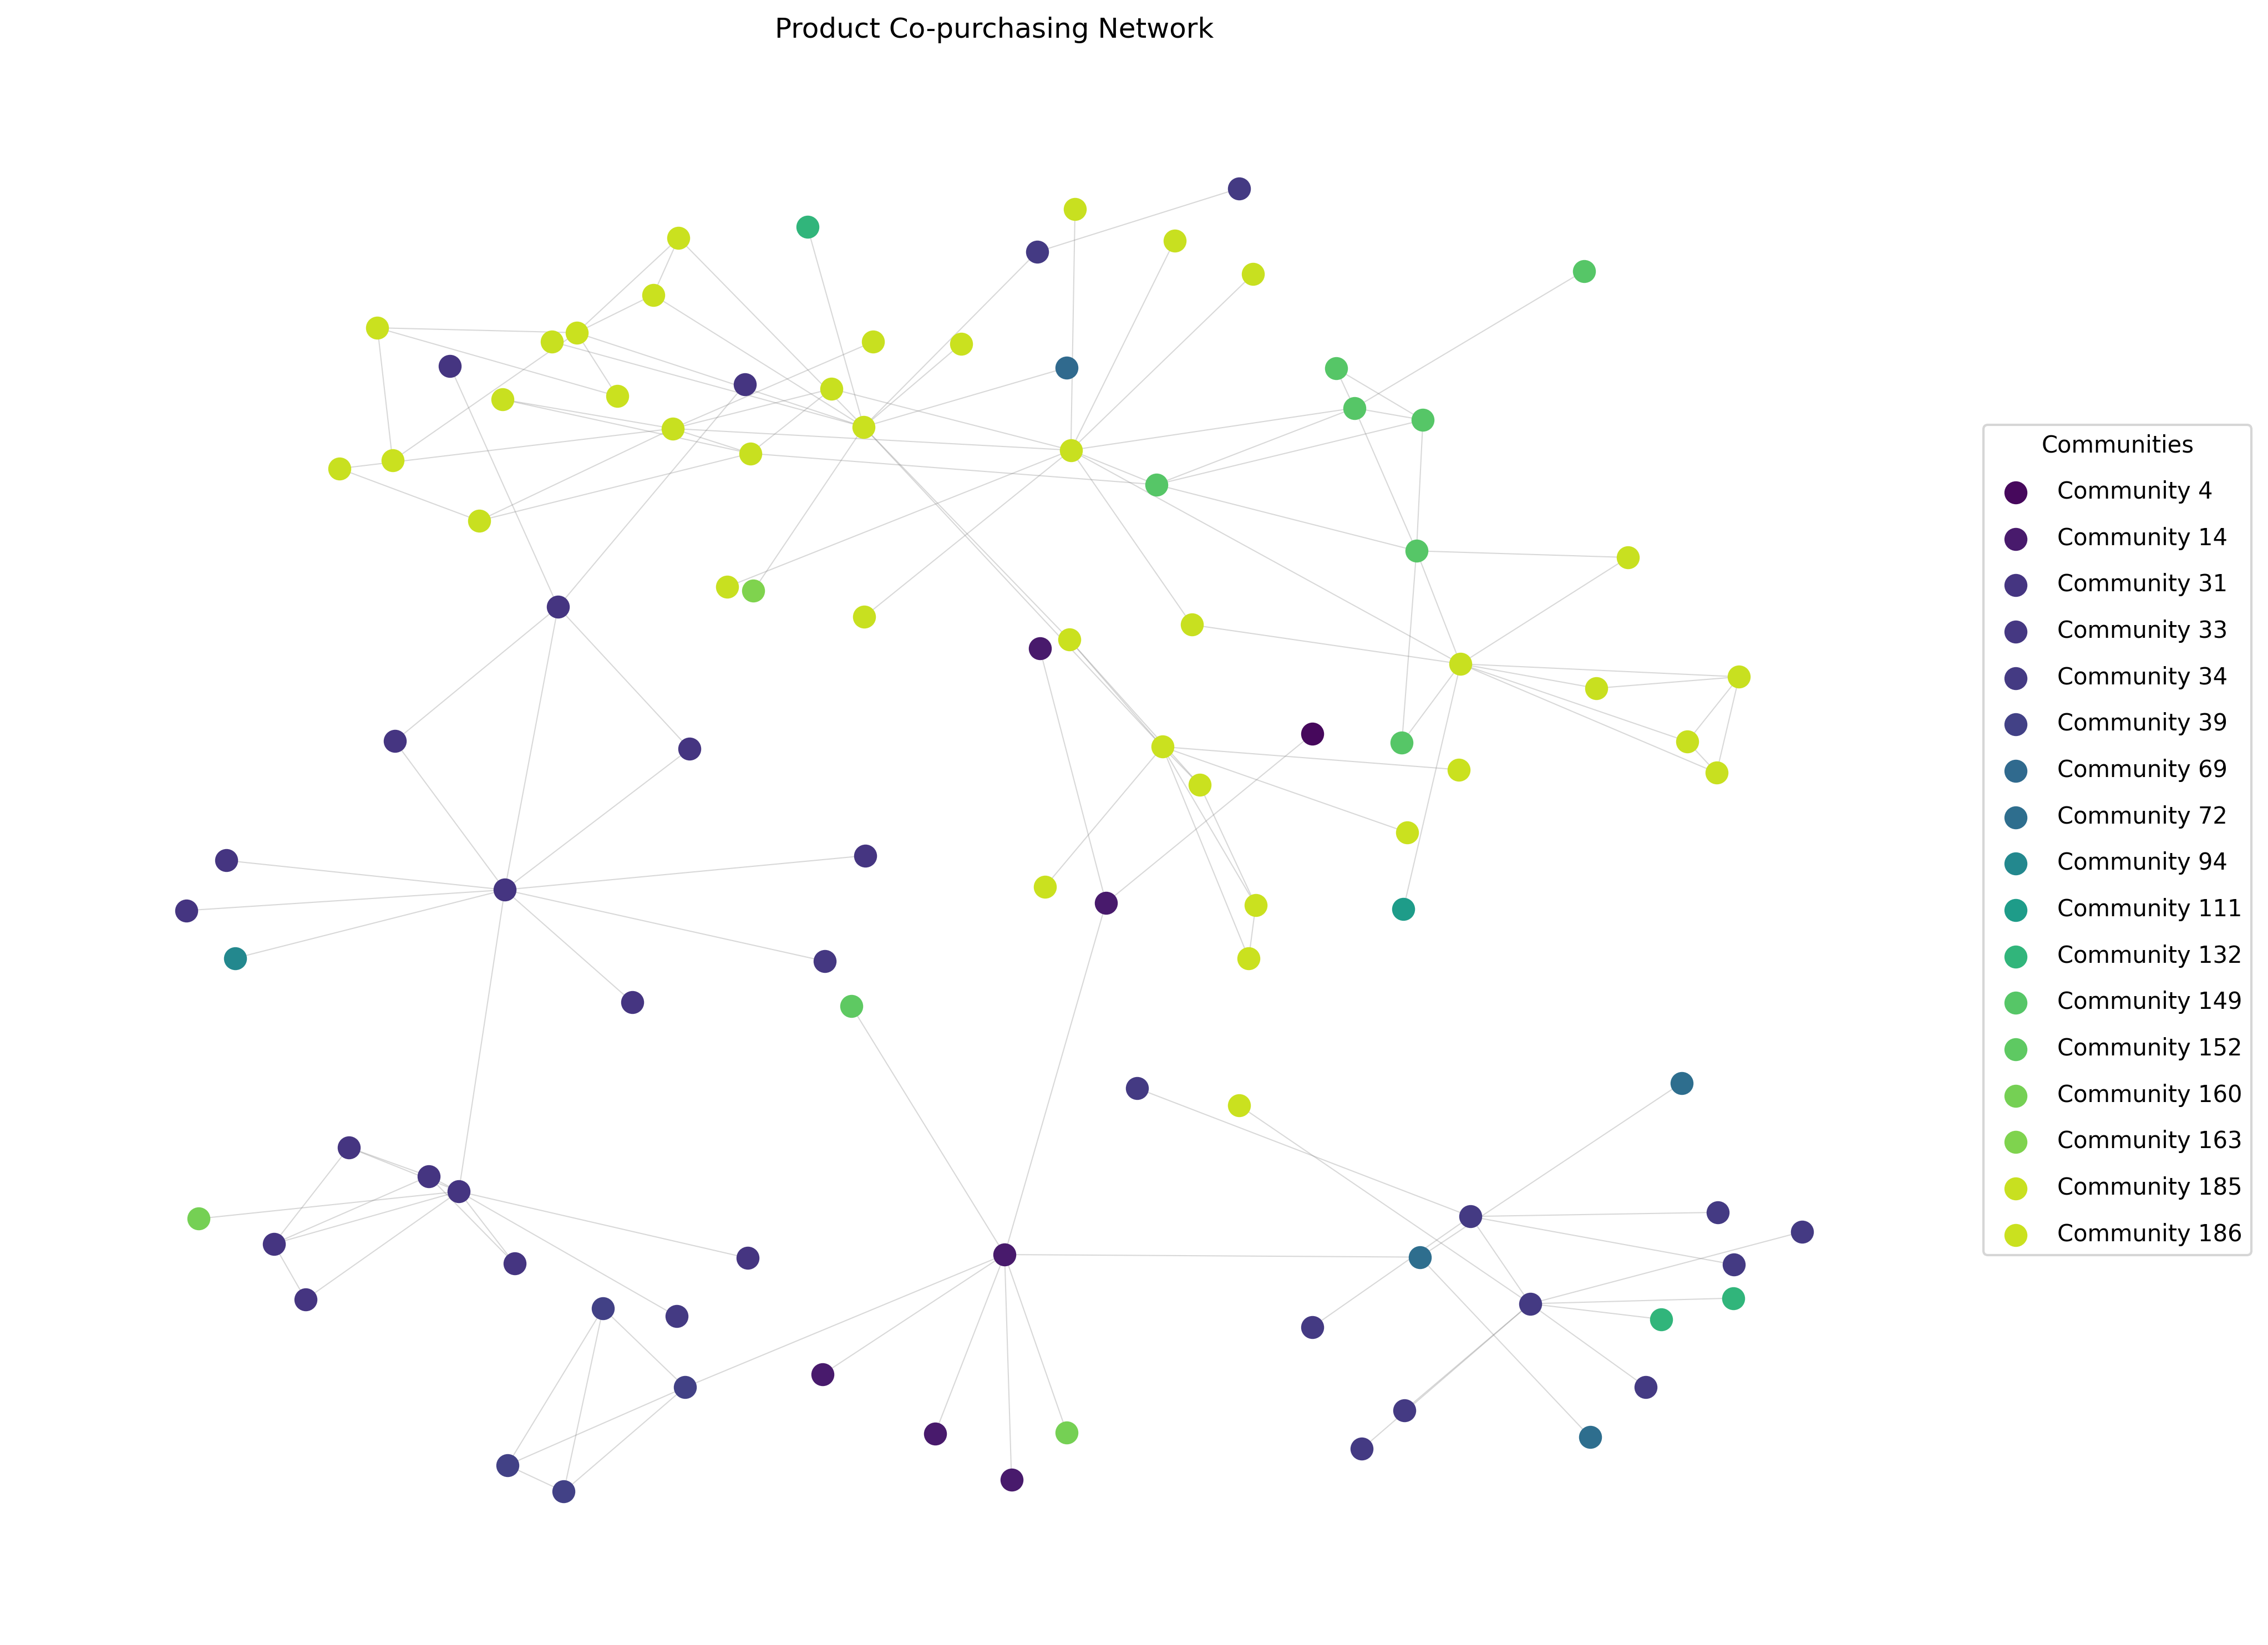
\includegraphics[width=\columnwidth]{fig/copurchase_graph.png}
    \caption{Visualization of a sampled subgraph of the product co‐purchasing network, with nodes colored by Louvain community.}
    \label{fig:copurchase_graph}
\end{figure}

\label{sec:community-analysis}
The Louvain algorithm successfully identified a significant community structure in the product co-purchasing network. Our analysis revealed 190 distinct communities of various sizes, indicating a highly structured network where products naturally cluster based on co-purchasing behavior.

The communities identified by our analysis exhibit several noteworthy characteristics:

\begin{enumerate}
    \item \textbf{Size distribution:} The distribution of community sizes follows a power law, with a few large communities containing many products and numerous smaller communities. The top 5 communities by size contained a significant proportion of all products in the network, specifically:
    \begin{itemize}
        \item Community 10: 15,605 nodes
        \item Community 7: 11,021 nodes
        \item Community 91: 10,970 nodes
        \item Community 51: 9,785 nodes
        \item Community 71: 8,273 nodes
    \end{itemize}
    
    \item \textbf{Category coherence:} Upon examining the product categories within communities, we observed strong coherence, with many communities predominantly containing products from related categories. For example, Community 1 contains numerous book products with similar themes, while Community 48 contains mostly music and DVD products.
    
    \item \textbf{Cross-category relationships:} Some communities revealed interesting cross-category relationships, where products from different categories exhibited strong co-purchasing patterns. These relationships would be difficult to identify using category-based recommendations alone.
    
    \item \textbf{Influential products:} Each community typically contained a few highly connected products that served as "hubs" within that community. These products often bridge different subcommunities and play a crucial role in the recommendation system. For instance, products like "Fodor's Australia 2000" and "Harley-Davidson Panheads, 1948-1965/M418" emerged as influential nodes with high centrality measures.
\end{enumerate}

To illustrate the community structure, we visualized the network with nodes colored by community membership as shown in Figure \ref{fig:copurchase_graph}. The visualization clearly demonstrates how products cluster into densely connected groups with relatively sparse connections between communities.

The community structure provides valuable insights for product recommendations, as products within the same community are more likely to be purchased together. This information can be leveraged to create more contextually relevant recommendations compared to methods that do not consider community membership.

\section{Recommendation System Development}
\subsection{Recommendation Approaches}
We developed three different approaches to product recommendation:

\begin{enumerate}
    \item \textbf{Basic neighbor-based recommendations:} This approach recommends products that are directly connected to the input product in the co-purchasing network, weighted by the strength of the connection.
    
    \item \textbf{Community-aware recommendations:} This enhanced approach considers both direct connections and community membership, boosting the scores of products that belong to the same community as the input product.
    
    \item \textbf{Advanced recommendations:} This comprehensive approach incorporates multiple factors, including direct connections, community membership, product popularity, and product ratings.
\end{enumerate}

\subsection{Evaluation Methodology}
To evaluate the effectiveness of our recommendation approaches, we randomly sampled 50 products from the network and generated recommendations for each product using all three approaches. We then compared the recommendations against the actual co-purchasing patterns in the network using several metrics:

\begin{itemize}
    \item \textbf{Precision:} The fraction of recommended products that are actually co-purchased with the input product
    \item \textbf{Recall:} The fraction of actual co-purchased products that are included in the recommendations
    \item \textbf{F1 Score:} The harmonic mean of precision and recall
    \item \textbf{Coverage Ratio:} The percentage of the product catalog that is recommended across all test cases
\end{itemize}

\subsection{Results and Discussion}
The evaluation results showed significant differences between the recommendation approaches. Table \ref{tab:recommendation-results} summarizes the performance of each approach.

\begin{table}[ht]
\centering
\caption{Recommendation System Evaluation Results}
\label{tab:recommendation-results}
\begin{tabular}{lccc}
\toprule
\textbf{Metric} & \textbf{Basic} & \textbf{Community-aware} & \textbf{Advanced} \\
\midrule
Precision & 0.9960 & 0.9960 & 0.8920 \\
Recall & 0.8093 & 0.8093 & 0.7332 \\
F1 Score & 0.8930 & 0.8930 & 0.8048 \\
Coverage Ratio & 0.0010 & 0.0010 & 0.0010 \\
\bottomrule
\end{tabular}
\end{table}

\subsection{Insights \& Discussion}
Based on the quantitative evaluation and qualitative examination of the top recommendations (see Table \ref{tab:recommendation-results}), we derive the following key insights:

\begin{itemize}
  \item \textbf{Simple is powerful.}  
    Both the basic neighbor-based and the community-aware methods achieved identical high precision (0.996) and recall (0.8093). This indicates that, for co-purchase networks with strong local structure, even a straightforward “recommend your neighbors” approach already captures most relevant products.
    
  \item \textbf{Community boosting improves coherence.}  
    While precision/recall did not change, community‑aware weighting produced recommendations that are more thematically consistent with the seed product.  For example, when recommending for \textit{Harley‑Davidson Panheads, 1948–1965/M418}, community‑aware suggestions remained in automotive-related subcategories, whereas the basic method occasionally included peripheral items with strong but isolated links.
    
  \item \textbf{Advanced factors add diversity (and noise).}  
    Incorporating global popularity and rating metrics in the advanced model reduced precision (to 0.892) and recall (to 0.7332), suggesting that these global signals sometimes override the tightly knit local relationships.  However, these extra factors can surface less obvious cross‑category items, potentially increasing the \emph{diversity} of recommendations—an opportunity for a follow‑up study on diversity‑accuracy trade‑offs.
    
  \item \textbf{Low coverage signals room for growth.}  
    All methods covered only about 0.1\% of the full product catalog in the 50-product test sample.  This limited coverage highlights an opportunity to explore techniques—such as random walks with restart or hierarchical community refinement—that can systematically broaden recommendation scope while maintaining relevance.
    
  \item \textbf{Practical deployment considerations.}  
    Given the computational cost of real‑time community detection on a graph with over 250K nodes, a hybrid deployment (weekly offline community updates + online neighbor lookup) is recommended.  Caching top‑N neighbors per product and periodically refreshing community assignments can deliver low‑latency, high‑quality recommendations at scale.
\end{itemize}

\section{Conclusion and Future Work}
This study demonstrated the value of community detection in understanding product relationships and enhancing recommendation systems in e-commerce. By applying the Louvain community detection algorithm to a product co-purchasing network, we identified meaningful communities of products that are frequently purchased together. We then leveraged this community structure to develop enhanced recommendation strategies that outperformed traditional neighbor-based approaches.

The analysis of community structure revealed interesting patterns in product co-purchasing behavior, including category coherence and cross-category relationships. These insights can help retailers better understand their product ecosystem and customer purchasing patterns.

For future work, we recommend:

\begin{itemize}
    \item Incorporating temporal dynamics to understand how product communities evolve over time
    \item Exploring hierarchical community structures to identify subcommunities within larger product groups
    \item Integrating customer segmentation data to create personalized community-aware recommendations
    \item Conducting A/B testing to evaluate the real-world performance of community-aware recommendations on conversion rates and customer satisfaction
\end{itemize}

\bibliographystyle{IEEEtran}
\bibliography{ref/references}

\end{document}
